\documentclass{llncs}

\usepackage[utf8]{inputenc}
\usepackage[english]{babel}

\usepackage{amsmath,amsfonts,amssymb}
\usepackage{array}
\usepackage{url}

\usepackage{tikz,pgfplots}

\tikzset{
  baseline=(current bounding box.center)
}

\newcommand{\doctype}{Parallel Radix Sort on OpenCL}

\usepackage{hyperref}
\hypersetup{
  breaklinks=true,
  colorlinks=true,
  citecolor=blue,
  linkcolor=blue,
  urlcolor=blue,
  bookmarksnumbered,
  bookmarksopen,
  pdftitle={\doctype},
  pdfauthor={Hennadiy Yatskov, Nico Mürdter},
  pdfsubject={},
  pdfkeywords={},
}

% Final Submit TODO: remove following line which makes margins smaller
\hypersetup{pdfpagescrop={92 62 523 748}}

\usepackage{breakurl}

\title{\doctype}
\author{Hennadiy Yatskov\\ Nico Mürdter}
\institute{
Karlsruhe Institute of Technology, Karlsruhe, Germany\\
\email{hennadiy.yatskov@student.kit.edu\\ nico.muerdter@student.kit.edu}}

\begin{document}

%% sp-process: load data in sql-table 'stats'
% IMPORT-DATA stats ../run.log

%% DEFMACRO REFORMAT(precision=0)
%% SELECT MAX(it) AS iterationcnt FROM stats
\def\iterationcnt{5}

\maketitle

\begin{abstract}
TODO
\end{abstract}

% Final Submit TODO: remove this prior to FINAL submission
\pagestyle{plain}

\section{Algorithm}
The algorithm is based on an open source implementation of P. Helluy \cite{ocl-radix-helluy}. It is seperated into three different phases, which are executed consecutively.

%TODO{Können wir wirklich auch negative integer sortieren????}
Before we come to the detailed explanation of the algorithm, we first need to define several values. $K(j)$ for $j=0 \dots N-1$, represents the non-sorted input values which consist only of integers. Each of these integers $K(j)$ is between $0$ and $2^b - 1$ and will be called a \textit{key} in the further explanation. Furthermore is the Radix represented by $R = 2^r$ where $r$ is the number of bits necessary representing $R$. We suppose thath $b$ is divisible by $r$ and so the number of passes is denoted by $p = b/r$. This assumption can be satisfied by an appropriate definition of $r$.

%If the number of elements in $K$ can't satisfy this assertion, it will be extended with maximum integer values so that is satisfies it. This extension is done with maximum values, so that the sorting is only influenced in the first phase of the algorithm, which will be explained in the next sections.

Each pass $q=0 \dots p-1$ of the algorithm consists in sorting the list according to the $q^{th}$ digit (in base $R$) $K(j)_q$. It is important to say, that each pass sorts the corresponding elements in a stable manner. So the work done in each pass is not corrupted by previous passes and will not corrupt following passes.

\subsection{Histograming}
This first phase of the algorithm is in charge of calculating the so called \textit{Histograms}. A histogram represents the number of occuring Radix in the given list of elements $K$. To do this fully parallel, the porcessing units are seperated in Groups $G$ with Items $I$, where an Item represents a Processor. So based on a GPU Architecture, the total amount of available Processing Units is $GI$. For the explanation we can suppose, that $N=GI$. If this is (most likely) not the case in a real scenario, the data can be extended by adding keys which represent the biggest possible value.

%TODO Geschickte Groupwahl etc noch einbringen.




\subsection{Scanning}

\subsection{Reordering}

\section{Implementation Details}

\subsection{Main Routine}

\subsection{Kernel}

\section{Experimental Results}

Your hardware.

What do you benchmark.

Running time~\ref{fi:runningtime:uniform} and speedup plots~\ref{fi:speedup:uniform} (for each generator, 64-bit integer and 32-bit floating point (not for  non-comparative integer sorting algorithms).

Interpretation.

\begin{figure}[h!]
\centering
\pgfplotsset{compat=1.5}
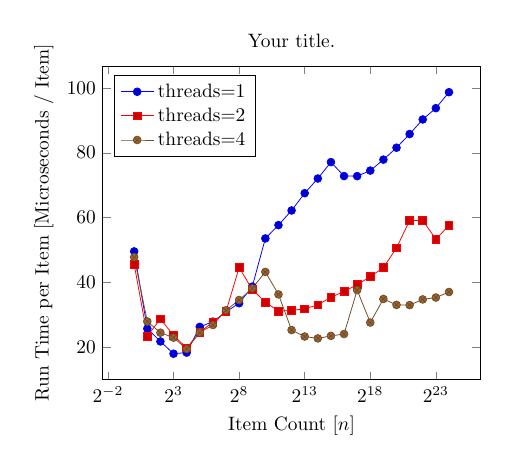
\begin{tikzpicture}[scale=0.7]
  \begin{axis}[
    title={Your title.},
    xlabel={Item Count [$n$]},
    ylabel={Run Time per Item [Microseconds / Item]},
    legend pos=north west,
    xmode=log,
    log basis x={2},
    ] 
    %% MULTIPLOT(threads) SELECT n AS x, (avg("wall-time") * 1.0 / n) AS y, MULTIPLOT
    %% FROM stats
    %% WHERE it > 0 AND "input-type"='uniform'
    %% GROUP BY MULTIPLOT,x ORDER BY MULTIPLOT,x
    \addplot coordinates { (1,49.6) (2,25.8) (4,21.85) (8,18.075) (16,18.4125) (32,26.3438) (64,27.9469) (128,30.9563) (256,33.6352) (512,38.7367) (1024,53.5891) (2048,57.7013) (4096,62.2103) (8192,67.5351) (16384,72.0565) (32768,77.1085) (65536,72.8129) (131072,72.7906) (262144,74.5003) (524288,77.8793) (1048576,81.5511) (2097152,85.7657) (4194304,90.2553) (8388608,93.7425) (16777216,98.6555) };
    \addlegendentry{threads=1};
    \addplot coordinates { (1,45.6) (2,23.5) (4,28.8) (8,23.675) (16,19.85) (32,24.75) (64,27.7625) (128,31.0453) (256,44.6383) (512,37.8852) (1024,33.967) (2048,31.1891) (4096,31.4354) (8192,31.9057) (16384,33.1395) (32768,35.4618) (65536,37.2686) (131072,39.349) (262144,41.8065) (524288,44.6163) (1048576,50.6581) (2097152,59.1302) (4194304,59.1624) (8388608,53.3066) (16777216,57.644) };
    \addlegendentry{threads=2};
    \addplot coordinates { (1,47.8) (2,28) (4,24.55) (8,23.025) (16,19.525) (32,24.5875) (64,26.925) (128,31.4609) (256,34.6203) (512,38.2023) (1024,43.274) (2048,36.3531) (4096,25.3622) (8192,23.3748) (16384,22.7897) (32768,23.568) (65536,24.1379) (131072,37.6677) (262144,27.6724) (524288,34.9413) (1048576,33.1177) (2097152,33.0524) (4194304,34.8011) (8388608,35.3875) (16777216,37.0874) };
    \addlegendentry{threads=4};
  \end{axis}
\end{tikzpicture}
\caption{Running times of \texttt{std::sort} with uniform input. Mean of \iterationcnt~iterations.}
\label{fi:runningtime:uniform}
\end{figure}


\begin{figure}[h!]
\centering
\pgfplotsset{compat=1.5}
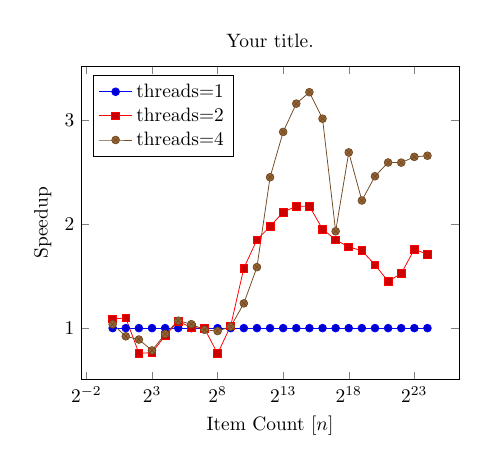
\begin{tikzpicture}[scale=0.7]
  \begin{axis}[
    title={Your title.},
    xlabel={Item Count [$n$]},
    ylabel={Speedup},
    legend pos=north west,
    xmode=log,
    log basis x={2},
    ] 
    %% MULTIPLOT(threads) SELECT s.n AS x, avg(s1."wall-time" * 1.0 / s1.n) / avg(s."wall-time" * 1.0 / s.n) AS y, s.threads
    %% FROM stats s CROSS JOIN stats s1
    %% WHERE s.it > 0
    %% AND s.it = s1.it
    %% AND s."input-type"='uniform'
    %% AND s."input-type" = s1."input-type"
    %% AND s.n = s1.n
    %% AND s1.threads=1
    %% GROUP BY s.threads,x ORDER BY s.threads,x
    \addplot coordinates { (1,1) (2,1) (4,1) (8,1) (16,1) (32,1) (64,1) (128,1) (256,1) (512,1) (1024,1) (2048,1) (4096,1) (8192,1) (16384,1) (32768,1) (65536,1) (131072,1) (262144,1) (524288,1) (1048576,1) (2097152,1) (4194304,1) (8388608,1) (16777216,1) };
    \addlegendentry{threads=1};
    \addplot coordinates { (1,1.08772) (2,1.09787) (4,0.758681) (8,0.763464) (16,0.927582) (32,1.06439) (64,1.00664) (128,0.997131) (256,0.753505) (512,1.02248) (1024,1.57768) (2048,1.85005) (4096,1.97898) (8192,2.11671) (16384,2.17434) (32768,2.17441) (65536,1.95373) (131072,1.84987) (262144,1.78203) (524288,1.74553) (1048576,1.60983) (2097152,1.45045) (4194304,1.52555) (8388608,1.75855) (16777216,1.71146) };
    \addlegendentry{threads=2};
    \addplot coordinates { (1,1.03766) (2,0.921429) (4,0.89002) (8,0.785016) (16,0.943022) (32,1.07143) (64,1.03795) (128,0.983958) (256,0.971544) (512,1.01399) (1024,1.23837) (2048,1.58724) (4096,2.45288) (8192,2.88923) (16384,3.1618) (32768,3.27174) (65536,3.01655) (131072,1.93244) (262144,2.69222) (524288,2.22886) (1048576,2.46246) (2097152,2.59484) (4194304,2.59346) (8388608,2.64903) (16777216,2.66008) };
    \addlegendentry{threads=4};
  \end{axis}
\end{tikzpicture}
\caption{Speedup of \texttt{std::sort} with uniform input. Mean of \iterationcnt~iterations.}
\label{fi:speedup:uniform}
\end{figure}

\begin{figure}[h!]
\centering
\pgfplotsset{compat=1.5}
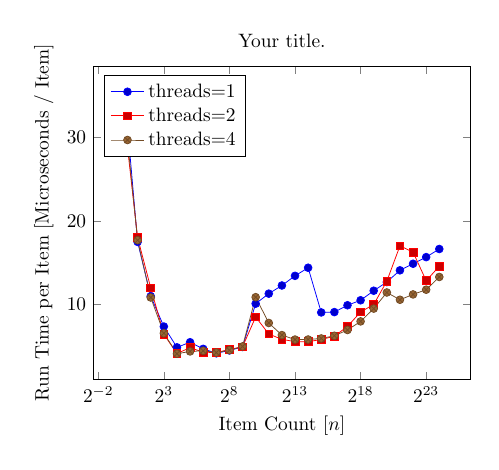
\begin{tikzpicture}[scale=0.7]
  \begin{axis}[
    title={Your title.},
    xlabel={Item Count [$n$]},
    ylabel={Run Time per Item [Microseconds / Item]},
    legend pos=north west,
    xmode=log,
    log basis x={2},
    ] 
    %% MULTIPLOT(threads) SELECT n AS x, (avg("wall-time") * 1.0 / n) AS y, MULTIPLOT
    %% FROM stats
    %% WHERE it > 0 AND "input-type"='zero'
    %% GROUP BY MULTIPLOT,x ORDER BY MULTIPLOT,x
    \addplot coordinates { (1,35.4) (2,17.5) (4,11) (8,7.375) (16,4.8875) (32,5.5) (64,4.70625) (128,4.17656) (256,4.52187) (512,4.93359) (1024,10.1123) (2048,11.3087) (4096,12.285) (8192,13.4385) (16384,14.4075) (32768,9.06262) (65536,9.10113) (131072,9.92058) (262144,10.5174) (524288,11.6572) (1048576,12.697) (2097152,14.0989) (4194304,14.8846) (8388608,15.6793) (16777216,16.6486) };
    \addlegendentry{threads=1};
    \addplot coordinates { (1,32) (2,18) (4,12) (8,6.45) (16,4.15) (32,4.85) (64,4.31562) (128,4.25469) (256,4.63438) (512,4.95469) (1024,8.52012) (2048,6.48506) (4096,5.8459) (8192,5.56848) (16384,5.56641) (32768,5.82274) (65536,6.21688) (131072,7.38593) (262144,9.11596) (524288,10.0179) (1048576,12.7968) (2097152,17.0248) (4194304,16.2725) (8388608,12.8521) (16777216,14.5902) };
    \addlegendentry{threads=2};
    \addplot coordinates { (1,33.2) (2,17.7) (4,10.85) (8,6.575) (16,4.125) (32,4.4) (64,4.475) (128,4.26562) (256,4.55234) (512,4.99922) (1024,10.8869) (2048,7.80156) (4096,6.35278) (8192,5.81973) (16384,5.82494) (32768,5.95208) (65536,6.27304) (131072,6.96391) (262144,7.99113) (524288,9.5204) (1048576,11.4477) (2097152,10.5781) (4194304,11.2183) (8388608,11.781) (16777216,13.3048) };
    \addlegendentry{threads=4};
  \end{axis}
\end{tikzpicture}
\caption{Running times of \texttt{std::sort} with zero input. Mean of \iterationcnt~iterations.}
\label{fi:runningtime:zero}
\end{figure}


\begin{figure}[h!]
\centering
\pgfplotsset{compat=1.5}
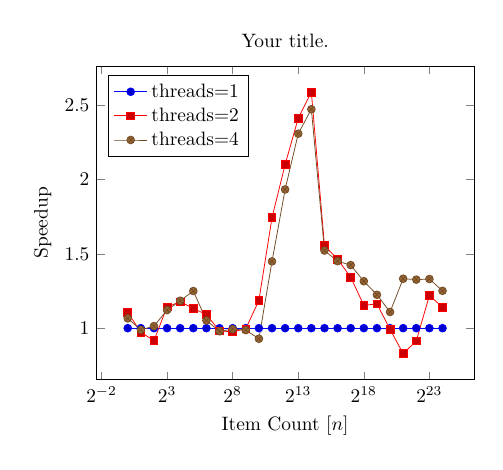
\begin{tikzpicture}[scale=0.7]
  \begin{axis}[
    title={Your title.},
    xlabel={Item Count [$n$]},
    ylabel={Speedup},
    legend pos=north west,
    xmode=log,
    log basis x={2},
    ] 
    %% MULTIPLOT(threads) SELECT s.n AS x, avg(s1."wall-time" * 1.0 / s1.n) / avg(s."wall-time" * 1.0 / s.n) AS y, s.threads
    %% FROM stats s CROSS JOIN stats s1
    %% WHERE s.it > 0
    %% AND s.it = s1.it
    %% AND s."input-type"='zero'
    %% AND s."input-type" = s1."input-type"
    %% AND s.n = s1.n
    %% AND s1.threads=1
    %% GROUP BY s.threads,x ORDER BY s.threads,x
    \addplot coordinates { (1,1) (2,1) (4,1) (8,1) (16,1) (32,1) (64,1) (128,1) (256,1) (512,1) (1024,1) (2048,1) (4096,1) (8192,1) (16384,1) (32768,1) (65536,1) (131072,1) (262144,1) (524288,1) (1048576,1) (2097152,1) (4194304,1) (8388608,1) (16777216,1) };
    \addlegendentry{threads=1};
    \addplot coordinates { (1,1.10625) (2,0.972222) (4,0.916667) (8,1.14341) (16,1.17771) (32,1.13402) (64,1.09051) (128,0.981638) (256,0.975725) (512,0.995743) (1024,1.18687) (2048,1.74381) (4096,2.10147) (8192,2.41331) (16384,2.58829) (32768,1.55642) (65536,1.46394) (131072,1.34317) (262144,1.15373) (524288,1.16363) (1048576,0.992201) (2097152,0.828136) (4194304,0.914709) (8388608,1.21998) (16777216,1.14108) };
    \addlegendentry{threads=2};
    \addplot coordinates { (1,1.06627) (2,0.988701) (4,1.01382) (8,1.12167) (16,1.18485) (32,1.25) (64,1.05168) (128,0.979121) (256,0.993307) (512,0.986873) (1024,0.92885) (2048,1.44954) (4096,1.93379) (8192,2.30912) (16384,2.47341) (32768,1.5226) (65536,1.45083) (131072,1.42457) (262144,1.31613) (524288,1.22444) (1048576,1.10913) (2097152,1.33284) (4194304,1.32681) (8388608,1.3309) (16777216,1.25133) };
    \addlegendentry{threads=4};

  \end{axis}
\end{tikzpicture}
\caption{Speedup of \texttt{std::sort} with zero input. Mean of \iterationcnt~iterations.}
\label{fi:speedup:zero}
\end{figure}

\bibliographystyle{splncs03}
\bibliography{sources}

\end{document}
